\chapter[Herausforderungen]{Herausforderungen}

Anschließend an die Beschreibung einer datengesteuerten Organisation, dessen Aufbau, Prozesse und Rollen, werden in diesem Kapitel die Herausforderungen zur Transformation in eine datengesteuerte Organisation thematisiert.

Bereits durch das äußere, sich schnell wechselnde kompetitive Umfeld einer Organisation, verkompliziert sich der Prozess datengesteuert z. B. Strategieentscheidungen in Organisation zu treffen. \footcite[Vgl.][S. 2]{Pratt.2023} 
Zusätzlich zu der Geschwindigkeit der Geschäftsumgebung, konnte durch eine Gartner Umfrage festgestellt werden, dass 65 \% der Teilnehmenden im Zeitraum der letzten zwei Jahre (2021-2023) einen Zuwachs der Komplexität von Entscheidungen verzeichneten. \footcite[Vgl.][S. 65]{Pratt.2023}
Damit ist das datengestützte Ableiten von Strategieentscheidungen ein besonders herausforderndes Feld aufgrund der hoch diversen Daten und der Vielzahl von Einflussvariablen. \footcite[Vgl.][S. 3]{Pratt.2023}
Diese äußeren Einflüsse wirken sich ebenfalls erschwerend auf interne managementbezogene und kulturelle Herausforderungen des Transformationsprozesses aus. \footcite[Vgl.][S. 15]{Dalpiaz.2020}
Bestätigt wird dies durch die Forschungsergebnisse von \Citeauthor*{Dalpiaz.2020}, welche 15 Interviews aus neun verschiedenen Softwareunternehmen auswerteten.
Aus den Interviews konnten die folgenden in Abbildung 4.1 dargelegte Herausforderungen in der Transformation zu einer datengesteuerten Organisation identifiziert werden. \footcite[][S. 9]{Dalpiaz.2020}

\begin{figure}[htb]
    \centering
    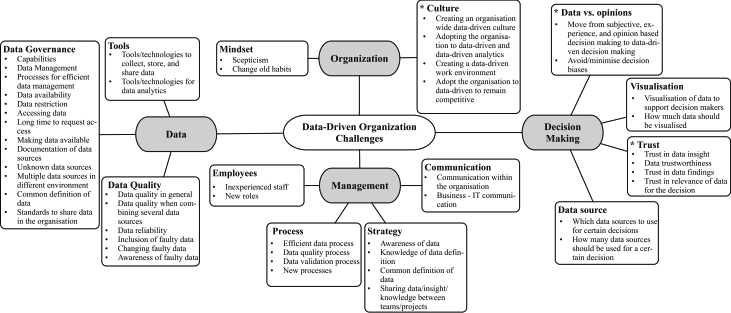
\includegraphics[width=0.95\textwidth]{graphics/DDO challenges.png}
    \caption{Herausforderungen einer datengesteuerten Organisation}
    \label{fig:DDOs challenges}
\end{figure}

Innerhalb der Grafik sind mittels \textbf{*} die drei wichtigsten Herausforderungen gekennzeichnet, welche alle 15 Teilnehmenden benannten: faktenbasierte Entscheidungen, Vertrauen und Kultur.
Faktenbasierte Entscheidungen beschreiben die Absicht, subjektive, erfahrungsgestützte und meinungsbasierte Entscheidungen durch die Nutzung von Daten durchzuführen oder bisherige Prozesse zu unterstützen. \footcite[Vgl.][S. 9]{Dalpiaz.2020}
Ein Einfluss auf die Umsetzung nimmt die zweite Herausforderung des Vertrauens.
Für faktenbasierte Entscheidungen ist ein hohes Maß an Vertrauen gegenüber vielerlei Aspekte der Daten, entlang des Data Science Prozesses, notwendig.
Diese Aspekte umfassen die Aufnahme relevanter Daten, die fehlerfreie Aufnahme der Daten, die fehlerlose Verarbeitung der Daten sowie die korrekte Ableitung von für die Entscheidung relevanten Erkenntnissen. \footcite[Vgl.][S. 10]{Dalpiaz.2020}
Die Aufnahme relevanter Daten wird dadurch herausfordernd, dass in etwa 10 \% der Daten insgesamt 90 \% des strategischen Werts enthalten. \footcite[Vgl.][S. 3]{Pratt.2023}
Neben der Geschäftsleitung ist ein Vertrauen gegenüber Daten und dessen Auswertung auch als gelebte Kultur der Organisation notwendig. \footcite[Vgl.][S. 4]{Dalpiaz.2020}
Eine gelebte datengesteuerte Kultur kann durch eine geringe Akzeptanz neuer Softwaretools und neuer Arbeitsmethoden verhindert werden. \footcite[Vgl.][S. 15]{Dalpiaz.2020}

Eine notwendige Tool gestützte Arbeitsweise ist z. B. die Dokumentation der Zusammenarbeit innerhalb des Teams und mit anderen Abteilungen. \footcite[Vgl.][S. 12]{Zhang.2020b}
Innerhalb dieser Dokumentation können z. B. Lösungen für technische Herausforderungen von der Datenbeschaffung bis zum Modelleinsatz festgehalten werden. \footcite[Vgl.][S. 23]{Grossman.2014}
Im Kontext von großen Datenumgebungen müssen technische Herausforderungen gelöst werden, welche zum einen die Aufnahme aller Daten betreffen. \footcite[Vgl.][S. 217]{Elgendy.2014}
Zum anderen ist die Flexibilität zu gewährleisten, neue Datenquellen einfach anzubinden und Auswertungen schnell durchführen zu können. \footcite[Vgl.][S. 217]{Elgendy.2014}
Durch Hinzunahme von Technologien, wie maschinelles Lernen zur Auswertung von Daten steigen ebenfalls die technischen Herausforderungen.
Maschinelles Lernen bedarf Testsysteme zum Einsatz von Modellen, anpassbare Software zur Überwachung der Modellleistung und Möglichkeiten zur Erläuterung der Modellergebnisse. \footcite[Vgl.][S. 1]{Nahar.2022}

Im gesamten Verlauf der Datenbeschaffung, Modellentwicklung und Ableitung von neuen Optimierungsprozessen sind diverse Teams erforderlich, um vorurteilsbehaftete Datenverarbeitung zu vermeiden. \footcite[Vgl.][S. 18]{Zhang.2020b}
Die Beschaffung von Arbeitskräften für ein solches diverses Team stellt eine weitere Herausforderung dar. 
Hierfür werden Bewerber mit datenbezogener Vergangenheit aus unterschiedlichen Branchen, oder Universitätsabsolventen und ein ausgearbeitetes Einarbeitungsprogramm benötigt. \footcite[Vgl.][S. 13]{Patil.2011}

Diese Herausforderung allein, sowie in Kombination mit den anderen thematisierten Herausforderungen bedarf eines Rahmenprogramms zur Integration von Data Science in verschiedenste Institutionen. \footcite[Vgl.][S. 1]{Saltz.2017}
